\chapter{Special topics for Developers}

\section{Authentication}
\label{cap:authentication}

In order to access API one need to authenticate itself. \zway uses sessions
to authenticate users. \zway session is called \textbf{ZWAYSession}.

If remote access is used, the find.z-wave.me service will issue an additional token called \textbf{ZBW\_SESSID}.

Please read in \ref{cap:authentication_usage} about the token lifetime, permanent tokens and token usage guide before selecting your preferred authentication method.

\subsection{Local authentication}
\label{cap:authentication_local}

If used in local network, \zway can be directly addressed via \murl{http://IP:8083}

Note that if \zway is used in trusted network and only \zwave API is supposed to be used, you might consider to skip authentication and check option \textit{Public API access} in \zwave Binding app.

\zway session can be obtained by sending login and password
in JSON format using POST to URL \murl{/ZAutomation/api/v1/login}
User credentials should look like \texttt{\{"login":"admin", "password":"admin"\}}.

It is also possible to use Basic Authentication to transmit login and password.

In return the session will be sent in three forms:
\begin{itemize}
\item as \textbf{data.sid} field in JSON structure (only for login using JSON),
\item as a header called \textbf{ZWAYSession},
\item as a cookie called \textbf{ZWAYSession}.
\end{itemize}

Example of successful login will look like:
\begin{listingverbatim}[Successful login reply]
{
    "data": {
        "sid": "ba69cb5b-b2fd-5ce0-5b75-9bae3e8bc369",
        "id": 1,
        "role": 1,
        "name": "Administrator",
        "lang": "en",
        "color": "#dddddd",
        "dashboard": [],
        "interval": 2000,
        "rooms": [
            0
        ],
        "hide_all_device_events": false,
        "hide_system_events": false,
        "hide_single_device_events": []
    },
    "code": 200,
    "message": "200 OK",
    "error": null
}
\end{listingverbatim}

\begin{listingverbatim}[Wrong login/password reply]
{
    "data": null,
    "code": 401,
    "message": "401 Unauthorized",
    "error": "User login/password is wrong."
}
\end{listingverbatim}

Once obtained, the session can be sent to the \zway server via the following ways:
\begin{itemize}
\item as an HTTP header called \textbf{ZWAYSession},
\item as a cookie called \textbf{ZWAYSession},
\item as an HTTP Authentication Bearer header (see \ref{cap:authentication_usage})
\end{itemize}

Below are few examples of local authentication.

With cURL using Authentication Bearer token:
{\scriptsize
\begin{quote} 
\cmdline{curl -H "Authorization: Bearer .../..." http://192.168.0.62:8083/ZAutomation/api/v1/...}
\end{quote}
}

With cURL using cookies:
{\scriptsize
\begin{quote} 
\cmdline{curl -H "Accept: application/json" -H "Content-Type: application/json" -X POST -d '\{"form": true, "login": "admin", "password": "admin"\}' http://192.168.0.62:8083/ZAutomation/api/v1/login -c cookie.txt}
\cmdline{curl http://192.168.0.62:8083/ZAutomation/api/v1/... -b cookie.txt}
\end{quote}
}

With cURL using Basic Authentication:
{\scriptsize
\begin{quote} 
\cmdline{curl -u admin:admin http://192.168.0.62:8083/ZAutomation/api/v1/...}
\end{quote}
}

With wget using Basic Authentication:
{\scriptsize
\begin{quote} 
\cmdline{wget --auth-no-challenge --user=admin --password=pwd 192.168.0.62:8083/ZAutomation/api/v1/...}
\end{quote}
}

From the browser using jQuery and Basic Authentication:
\begin{listingverbatim}[Login with jQuery]
jQuery('img').click(function() {
    jQuery.ajax({
        url: "http://192.168.0.62:8083/ZAutomation/api/v1/...",
        beforeSend: function (xhr) { xhr.setRequestHeader ("Authorization", "Basic " + btoa("admin" + ":" + "password")); }
    });
});
\end{listingverbatim}

\subsection{Remote authentication}
\label{cap:authentication_remote}

If not disabled by the user, \zway provides remote access service to the controller via \murl{https://find.z-wave.me}
See section \ref{remoteaccess} for more information on the \zway remote access service.

This service accepts \zwaydeviceid, username and password, checks entered
credentials agains your \zway and if accepted returns back two sessions \textbf{ZWAYSession}
and \textbf{ZBW\_SESSID} in two forms:
\begin{itemize}
\item as a header,
\item as a cookie.
\end{itemize}

The session can be obtained by
\begin{itemize}
\item logging in the form on \murl{https://find.z-wave.me/zboxweb}
\item sending a POST request to \murl{https://find.z-wave.me/zboxweb} with form data \texttt{act=login\&login=id/admin\&pass=password}
\end{itemize}

\begin{figure}
\begin{center}
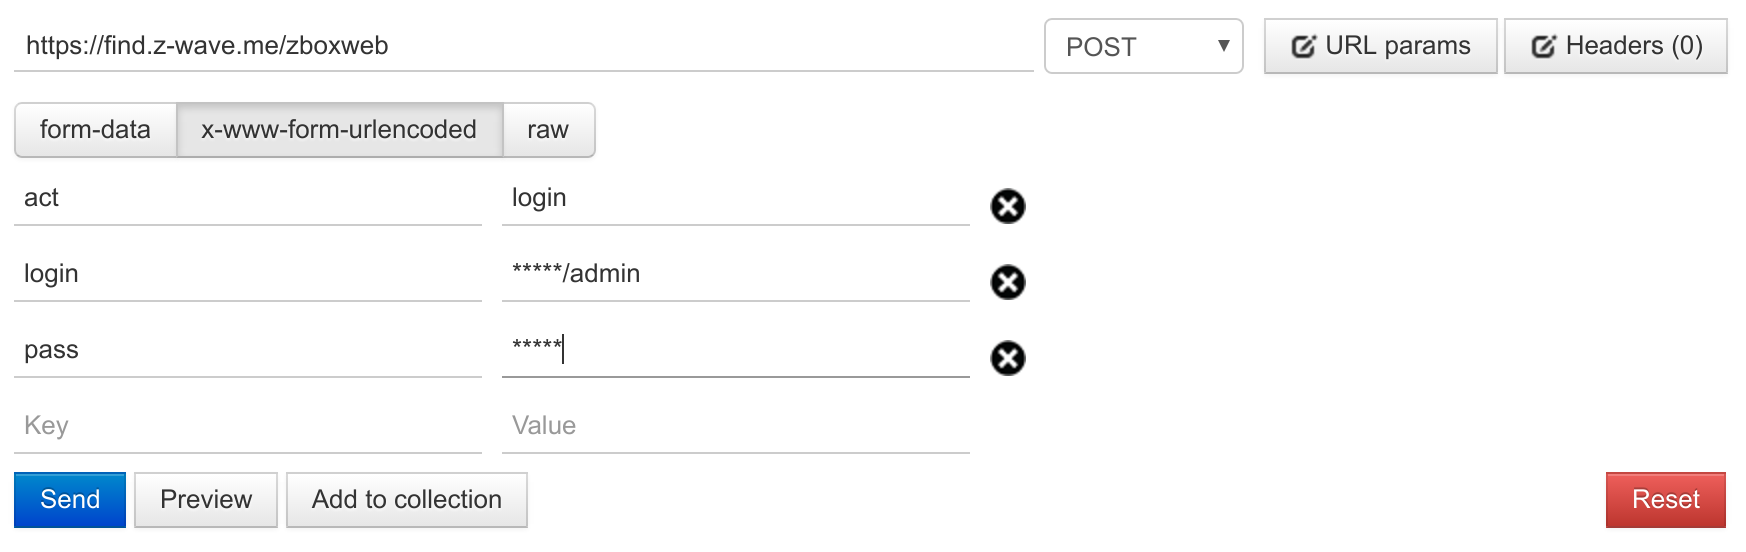
\includegraphics[width=0.7\textwidth]{pngs/cap13/find-login-postman.png}
\caption{Example of login on find.z-wave.me using Postman}
\label{authenticatioln_remote_find}
\end{center}
\end{figure}

Once logged in with \texttt{act=login}, the user is redirected to the / of the \zway (in most cases it then redirects to /smarthome/).
If you want the user to be redirected to some specific URL after log in add one more parameter \texttt{ruri=...} (see examples below).

The obtained session will be returned
\begin{itemize}
\item as an HTTP header,
\item as a cookie.
\end{itemize}

To suppress the redirect use \texttt{act=auth}.

The credential can be used in subsequent requests in one of the three forms listed below (in order they are checked in \zway):
\begin{itemize}
\item as HTTP \textbf{Authentication: Bearer} header (see below),
\item as HTTP \textbf{X-ZBW-SESSID} and \textbf{ZWAYSession} headers,
\item as \textbf{ZBW\_SESSID} and \textbf{ZWAYSession} cookies.
\end{itemize}

Below are examples of remote authentication.

With cURL using Authentication Bearer token:
{\scriptsize
\begin{quote} 
\cmdline{curl -H "Authorization: Bearer .../..." https://find.z-wave.me/ZAutomation/api/v1/...}
\end{quote}
}

With cURL using cookies:
{\scriptsize
\begin{quote} 
\cmdline{curl -H "Accept: application/json" -X POST -d 'act=login\&login=132339/admin\&pass=admin1' https://find.z-wave.me/zboxweb -c cookie.txt}
\cmdline{curl https://find.z-wave.me/ZAutomation/api/v1/... -b cookie.txt}
\end{quote}
}

%With cURL using cookies in one single command (with follow redirect):
%{\scriptsize
%\begin{quote} 
%\cmdline{curl -H "Accept: application/json" -X POST -d 'act=login\&login=132339/admin\&pass=admin1\&ruri=/ZAutomation/api/v1/devices' https://find.z-wave.me/zboxweb -c cookie.txt -b cookie.txt -L}
%\end{quote}
%}

If you want the user to be redirected to a specific page after login, you can also use the following url: \murl{https://find.z-wave.me/zboxweb?ruri=/expert} or \murl{https://find.z-wave.me/zboxweb?ruri=/expert&id=123456&login=admin} to pre-fill \zwaydeviceid and user name.

\subsection{Remote authentication and access error handling}
\label{cap:authentication_remote_errors}

The tables below describe possible errors returned by the remote access service. Errors are order exactly as the request is handled.

Authentication on \texttt{https://find.z-wave.me/zboxweb} with \texttt{act=login}: \\
\begin{tabular}{|p{0.25\textwidth}|p{0.1\textwidth}|p{0.65\textwidth}|}
\hline
Condition & HTTP code & Redirect URL \\
\hline
Box not connected to the server & 302 & \murl{https://find.z-wave.me/zboxweb?err=bad\_login&ruri=\%2F} \\
\hline
Box connected, but default login/password admin/admin is used & 302 & \murl{https://find.z-wave.me/zboxweb?err=insecure\_login\_pass&ruri=\%2F} \\
\hline
Box not connected to find.z-wave.me & 502 & \\
\hline
Box connected, but login/password is invalid & 302 & \murl{https://find.z-wave.me/zboxweb?err=bad\_login&ruri=\%2F} \\
\hline
Box connected and authentication is successful & 302 & \murl{https://find.z-wave.me/} \\
\hline
\end{tabular}

Authentication on \texttt{https://find.z-wave.me/zboxweb} with \texttt{act=auth}: \\
\begin{tabular}{|p{0.25\textwidth}|p{0.1\textwidth}|p{0.65\textwidth}|}
\hline
Condition & HTTP code & HTTP error message \\
\hline
Box not connected to the server & 403 & Forbidden \newline Wrong username or password \\
\hline
Box connected, but default login/password admin/admin is used & 403 & insecure\_login\_pass \newline Your (username, pass) pair is insecure \\
\hline
Box not connected to find.z-wave.me & 502 & \\
\hline
Box connected, but login/password is invalid & 403 & Forbidden \newline Wrong username or password \\
\hline
Box connected and authentication is successful & 200 & \\
\hline
\end{tabular}

Subsequent requests to \texttt{https://find.z-wave.me/PATH}, where \texttt{PATH} is not equal to \texttt{zboxweb} or \texttt{zboxweb/*}: \\
\begin{tabular}{|p{0.25\textwidth}|p{0.1\textwidth}|p{0.65\textwidth}|}
\hline
Condition & HTTP code & Redirect URL \\
\hline
No token (no Authorization header, no X-ZBW-SESSID header, no ZBW\_SESSID cookie) & 307 & \murl{https://find.z-wave.me/zboxweb/r//PATH} \\
\hline
Invalid token (incorrect or expired or revoked) & 307 & \murl{https://find.z-wave.me/zboxweb/r//PATH} \\
\hline
Box not connected to find.z-wave.me & 502 & \\
\hline
Server side error & 500 & \\
\hline
\end{tabular}

\subsection{Token lifetime}
\label{cap:authentication_usage}

Each time you log in using methods described above a new session is created. This session will live for one week (might be changed on \zway side and on find.z-wave.me side, do not rely on this period).

Those login methods are good to obtain the token once to the access the API via token or for rare single actions. Creating a new session each time will pollute user profile in \zway.

Tokens can be deleted at any time in User management (\ref{cap4:user_management}) panel. This will lead to log-out of the application that is using this token. This application will loose access to \zway and will require again a log in via username and password.

To use tokens long term we recommend to make them permanent. You can make any token permanent by pressing a button in User management (\ref{cap4:user_management}).
Permanent token do never expire until deleted. Only \zway token can be made permanent that way.

To make both find.z-wave.me and \zway token permanent use \textbf{Authentication Bearer} way to transmit tokens.

Both find.z-wave.me remote access service and \zway do support \textbf{Authentication Bearer} HTTP header. This header is commonly used in OAuth2 authentication protocol, but you can use it without OAuth2 too.

\zway and find.z-wave.me will automatically mark tokens as permanent if they are received in \textbf{Authentication Bearer} header.

The format of the header is: \texttt{Authorization: Bearer \textbf{ZBW\_SESSID}/\textbf{ZWAYSession}}.
Note that if direct access is needed (not via find.z-wave.me), \textbf{ZBW\_SESSID} can be omitted.
In this case a slash \textbf{/} should still preceed \textbf{ZWAYSession}

A typical application should take usename and password to log in via find.z-wave.me and get both \textbf{ZWAYSession} and \textbf{ZBW\_SESSID} tokens to form Authentication Bearer token.
The username and password should then be erased from the memory, while Authentication Bearer token should be saved for future use. It is not recommended to save user credentials.

Like other tokens user can delete the permanent token in the User management (\ref{cap4:user_management}) panel.

\subsection{OAuth2}
\label{cap:authentication_oauth2}

\zway do also support OAuth2 authentication method to provide access to smart home devices to third party services like voice assistances (Amazon Alexa, Google Home, Yandex Alice), IFTTT and some others.

To get integrated one should provide to the \zwaveme team redirect\_uri and get back OAuth2 server URL, client\_id and client\_secret. Please contact info@z-wave.me.

To let the user authenticate and grant access to his devices you should redirect him to one of the two pages:
\murl{https://z-wave.me/oauth2/?state=...\&redirect\_uri=https://...\&response\_type=code\&client_id=...}
\murl{https://find.z-wave.me/zboxweb?lang=...\&hide_diruris=1\&ruri=/smarthome/\%23/oauth2\%3Fstate\%3D...\%26redirect_uri\%3Dhttps\%3A\%2F\%2F...\%26response\_type\%3Dcode\%26client\_id\%3D...}

In this request:
\begin{itemize}
\item lang (optional --- English if omitted) — pre-selects the find.z-wave.me interface language (see ZBW\_IFLANG cookie for the correct value)
\item ruri --- URL encoded link to the target page in \zway user interface to OAuth2 page:
	\murl{/smarthome/\#/oauth2?state=...\&redirect\_uri=https://...\&response\_type=code\&client\_id=...}
\begin{itemize}
	\item state --- specific value used by your service to match the OAuth2 reply with the original request --- used with redirected to redirect\_uri
	\item redirect\_uri --- the URL to redirect the user to once the authorization was granted
	\item response\_type --- the type of OAuth2 authorization; only \textit{code} is currently supported
	\item client\_id --- id of the client that should match redirect\_uri on \zwaveme OAuth2 server.
\end{itemize}
\end{itemize}

After the user logs in to \zway he is asked to mark rooms and devices to be granted access to.
A new user will then be created with the corresponding permissions and a session token will be generated.
The session is saved on the \zwaveme OAuth2 server together with an authorization code.

On the next step the user is redirected back to the service using URL \murl{redirect\_uri?state=...&code=...}
In this request:
\begin{itemize}
\item state --- specific value used by your service to match the OAuth2 reply with the original request (see above)
\item code --- the authorization code to be used to get access token from the OAuth2 server
\end{itemize}

The service can now make a POST request to the \zwaveme OAuth2 server on \murl{/token} providing \texttt{client\_id}, \texttt{client\_secret} and \texttt{code}.
The request can use JSON format or form data or url encoded form. The response is a JSON with access\_token or error message.

The resulting access\_token is to be used in the Authentication Bearer HTTP header.
This token never expires unless deleted by the user.

\begin{listingverbatim}[Request of Access token via Authorization code (JSON format)]
Content-type: application/json
{
    "client_id": "...",
    "client_secret": "...",
    "code": "..."
}
\end{listingverbatim}

\begin{listingverbatim}[Request of Access token via Authorization code (URL encoded form)]
Content-Type: application/x-www-form-urlencoded
client_id=...&client_secret=...&code=... (URL encoded!)
\end{listingverbatim}

\begin{listingverbatim}[Request of Access token via Authorization code (form data)]
Content-Type: multipart/form-data; boundary=----WebKitFormBoundarytufRVLxOz9VdsQbA

------WebKitFormBoundarytufRVLxOz9VdsQbA
Content-Disposition: form-data; name="client_id"

...
------WebKitFormBoundarytufRVLxOz9VdsQbA
Content-Disposition: form-data; name="client_secret"

...
------WebKitFormBoundarytufRVLxOz9VdsQbA
Content-Disposition: form-data; name="code"

...
------WebKitFormBoundarytufRVLxOz9VdsQbA--
\end{listingverbatim}

\begin{listingverbatim}[Access token successfuly retrieved]
{
    "access_token": ".../...",
    "token_type": "bearer"
}
\end{listingverbatim}

\begin{listingverbatim}[Authorization code is invalid (400 Bad request)]
{
    "error": "invalid_grant"
}
\end{listingverbatim}

\begin{listingverbatim}[Wrong credentials (400 Bad request)]
{
    "error": "invalid_client"
}
\end{listingverbatim}


\section{How to write own Apps for \zway}
\label{developownapps}

According to Chapter \ref{cap:modules} apps have two core files:

\begin{itemize}
\item module.js
\item index.js
\end{itemize}

The following chapter explains these two files more in detail. 

\subsection{module.js}

Module.js defines the general behavior of the app and the interface to the user side.
Table \ref{tab:module.json} 
shows the structure of the file module.js with an explanation of each line item.

\begin{table}
\begin{tabular}{|p{0.45\textwidth}|p{0.5\textwidth}|}
\hline
\{ "singleton" : false, &
Boolean to set if there can be multiple Instances of the
module allowed or not \\
"dependencies": [], & 
An array list of all module names from which this module is dependent. Modules in this list
should be 'singleton'.Thew module cannot be instantiated if at least one of the modules
in the list does not have an instance. \\
\hline
"category": "automation\_basics", & 
The app category this module is shown in the app store. Known app store categories are:
'basic\_gateway\_modules',
'legacy\_products\_workaround', 'support\_external\_ui',
'support\_external\_dev', 'automation\_basic',
'device\_enhancements', 'developers\_stuff',
'complex\_applications', 'automation', 'security',
'peripherals', 'surveillance', 'logging', 'scripting',
'scheduling', 'climate', 'environment', 'scenes',
'notifications', 'tagging' \\
\hline
"author": "Z-Wave.Me", & Author name of the Module \\
\hline
"homepage": "http://razberry.z-wave.me", &
If you have a news homepage, it can be linked here. \\
\hline
"icon": "icon.png", & Name of the icon which is shown for this module
on the UI \\
\hline
"moduleName": "AppClassName", & Module name have to the same like the class
reference \\
\hline
"version": "1.0.0", &Version number of this module \\
\hline
"maturity": "beta", & Status if the app is still in development or released \\
\hline
"repository": \{ Repository optional "type": "git", Kind of the repository
"source":
https://github.com/ZWaveMe/homeautomation \}, &
Address of the repository \\
\hline
"defaults" : \{ "title" : "\_\_m\_title\_\_", & The title placeholder for the Language files \\
\hline
"description" : \{ "\_m\_descr\_\_" \}, &
The description placeholder for the language files \\
\hline
"schema" : \{\}, & Description of the data structure of the form for
instantiating the module. See explanation of schema for details \\
\hline
"options" : \{\}\} & Showing options of the setup form\\
\hline
"description" : \{ "\_m\_descr\_\_" \}, &
The description placeholder for the language files \\
\hline
\end{tabular}
\caption{Module.json details} 
\label{tab:module.json}
\end{table}	

\subsection{Schema}

The \textbf{schema} is a JSON Structure to define the user interface of the module.
It lists all input parameters and  options to be shown in the setup dialog of the app:

\begin{listingverbatim}[Schema Structure]
{
  "schema": {
    "type": "object",
    "properties": {
    }
  }
}
\end{listingverbatim}


The structure of the schema is the following. Inside the 'properties' space the single 'properties' 
can be defined. They become the parameter of the module during the initiation and they 
are shown as configuration parameters in the setup dialog. There are different
types of input parameters:


\subsubsection{Primitive data types like integer, float or string}

\begin{listingverbatim}[Schema Structure Simple Type]
{
  //Parametername
  "name": {
    "type": "array",
    "items": {
      "title": "Device",
      "type": "radio",
      //array of choosable items
      "enum": ["Adult", "Child"],
      "default": "Child",
      "required": true
    }
  },
  //Parametername
  "name": {
    "type": "integer",
    "required": true
  },
}
\end{listingverbatim}

\subsubsection{Name Spaces  - Enumerations with a choice}

\begin{listingverbatim}[Schema Structure Enumerations with a choice]
{
  //Parametername
  "name": {
    "field": "enum",
    "datasource": "namespaces",
    //special namespacedestination
    "enum": "namespaces:devices\_all:deviceId",
    "required": true
  },
}
\end{listingverbatim}



Name spaces refer to the internal \zway structure. It allows to list elements from 
the \zway data model and filter it. The statement 
\texttt{"namespaces:devices\_all:deviceId"} will offer a selection of all devices.

Namespaces can also be combined like

\murl{namespaces:devices\_doorlock:deviceId,namespaces:devices\_switchBinary:deviceId}

which means devices doorlock and all binary switches.
Namespaces can also be REST paths like

\murl{server:port/v1/namespaces/{devices\_DEVICETYPE}.{PATH}}


\subsection{The file index.js}

Thew file index.js contains the application as such. It can include other js files is needed 
but \zway will always look for a index.js file to load first. Table \ref{tab:detailindexjs}
list the basic structure of index.js with the minimum functions.


\begin{table}
\begin{tabular}{|p{0.45\textwidth}|p{0.5\textwidth}|}
\hline
\texttt{\tiny 
function AppClassName (id, controller) {AppClassName.super\_.call(this, id, controller);} }&
Constructor method:
This line is a call of the Superconstructor. It has always to be first line of the constructor \\
\hline
\texttt{\tiny inherits(AppClassName, AutomationModule); }
&
inheration call: \\
\hline
\texttt{\tiny \_module = AppClassName;} &
The definition of the class reference \\
\hline
\texttt{\tiny AppClassName.prototype.init = function (config) {
AppClassName.super\_.prototype.init.call(this, config);
var self = this; }; }&
Initialization method: Variable to refer to in the class in own
methods (this is context dependent in JavaScript).
Here you can register 'listeners' for the event bus. For details on event bus please 
refer to chapter \ref{cap:eventbus} \\
\hline

\texttt{\tiny AppClassName.prototype.stop = function () {
AppClassName.super\_.prototype.stop.call(this);}; }&
Destroy method:
Here you have to unregister 'listeners'.  \\
\hline
\texttt{\tiny AppClassName.prototype.Methodname=
function(parameter) }&
Own Methods: Write your own Methods here. \\
\hline
\end{tabular}
\caption{Details of index.js} 
\label{tab:detailindexjs}
\end{table}	
	

More information e.g. about the list of probe types etc. you find on 

\murl{http://docs.zwayhomeautomation.apiary.io/}

\section{Write you own Device Description Files}
\label {newddr} 

This part of the manual is not yet published because the service for creating own Device 
Description Files is not yet available.

\section{Extending EnOcean}
\label{addenocean}

How to include a new EnOcean Device (example Hoppe Door handle)

(1) Check if the profile is in \cmdline{/opt/z-way-server/config/Profile.xml}. Not that 
you just need to know the profile the given product supports. There is no way 
to find out automatically! 

\begin{listingverbatim}[EnOcean Profile Entry]
<Profile rorg="0xf6" func="0x10" type="0x00" rorgDescription="RPS Telegram"
    funcDescription="Mechanical Handle" typeDescription="Window Handle">
  <Field offset="0" size="4" name="windowHandle" type="int" description="Movement of the window handle" short="WIN" />
</Profile>
\end{listingverbatim}

(2) Add the device record of the device to 

{\small
\cmdline{/opt/z-wave-server/htdocs/smarthome/storage/data/devices\_encoean.json}. 
}
Here the rorg, funcid and type are set. Now the device record will be created and the 
right values are changed on message reception. Now you need to make sure the right  
element is rendered and updated. This is 
in \cmdline{/opt/z-wave-server/automation/modules/Enocean/index.js}

First add a filter to catch the events and call the correct function:

\begin{listingverbatim}[Catch Device IDs]
if (matchDevice(0xf6, 0x10, 0x01)) {
  // Hoppe Window handle
  windowHandle("contact", "window", "Windor Handle");
}
\end{listingverbatim}
now you add the function that handles the value changes and renders the element 
accordingly. For the window handle we use the binary sensor element but overwrite 
the status information according to the information of the window handle moves.  

\begin{listingverbatim}[Handle Device]
function windowHandle(dh, type, title) {
	var vDev = self.controller.devices.create({
	deviceId: vDevIdPrefix + type,
	defaults: {
		deviceType: 'sensorBinary',
		metrics: {
			probeTitle: type,
			scaleTitle: '',
			icon: type,
			level: '',
			title: title
		}
	},
	overlay: {},
	handler: function(command) {},
	moduleId: self.id
});

if (vDev) {
	self.dataBind(self.gateDataBinding, self.zeno, nodeId, dh, 
	function(type) {
		try {
			if (this. handleValue == 13)
				vDev.set("metrics:level", "tilt");
			if (this. handleValue == 15)
				vDev.set("metrics:level", "closed");
			if (this. handleValue == 12 || this. handleValue == 14)
				vDev.set("metrics:level", "open");
		} catch (e) {}
	}, "value");
}
}
\end{listingverbatim}